\documentclass[11pt]{article}
\usepackage[margin=0.85in]{geometry}
\usepackage{booktabs}
\usepackage{amsmath}
\usepackage{enumitem}
\usepackage{graphicx}
\usepackage[hidelinks]{hyperref}
\usepackage{titlesec}
\titlespacing*{\section}{0pt}{6pt}{2pt}
\titleformat*{\section}{\large\bfseries}

\setlist{nosep}
\setlength{\parskip}{4pt}
\setlength{\parindent}{0pt}

\title{ISyE 3133 Programming Assignment3: Improving the Final Exam Schedule}
\author{Kelechi Ejieke and Temidayo Solomon}
\date{\today}

\begin{document}
\maketitle
\vspace{-2.2em}

%--------------------------------------------------
\section{Problem and data}
We reschedule 24 ISyE sections for 360 students; reading/conflict periods and 7 external common exams stay fixed. Only 8 regular periods have rooms (P03, P05, P09, P14, P17, P21, P22, P23), giving 24 room-period slots with 3 rooms and 32 with the optional Klaus-2443. Three of the 8 periods fall on Dec 17, so the draft puts 9 exams on one day. Sections (54--66 students) always fit the smallest room (75), so none is split. All externals run 18:00--20:50; 210 students take one.

%--------------------------------------------------
\section{What makes a good schedule}
\textbf{Workload.} Each pair of \emph{consecutive} exams in a student's timeline (externals included) gets one penalty: 5 for a 30-minute back to back (P03$\to$P04, P21$\to$P22, P22$\to$P23), 3 for an evening exam followed by an 8am exam the next day, and 1 for two exams on one day with a long gap. A day with 3+ exams adds 10, so a full Dec 17 scores $5+5+10=20$. A back to back ranks worst because it leaves no time to rest or review; an overnight pair costs sleep but leaves time to eat and sleep. These weights are our judgment, not measured preferences.

\textbf{Disruption and tradeoff.} A \emph{move} is a section whose period differs from the draft. Room changes get weight 0.01, which can never outweigh one workload point. We minimize workload subject to at most $k$ moves for $k=0,\dots,24$, which traces the full workload--disruption frontier instead of fixing an arbitrary weight. We also report the worst-off student, students penalized, and students whose exam time changes.

%--------------------------------------------------
\section{Model}
Sets: sections $E$, rooms $R$, usable periods $P$, available pairs $A\subseteq R\times P$, students $S$, timeline periods $T\supseteq P$ (adds external periods), days $D$, courses $C$; $Q$ = penalized period pairs $(p,q)$ with weight $w_{pq}$ and periods strictly between them $B_{pq}$. Data: size $n_e$, capacity $c_r$, course $\kappa(e)$, sections $E_s$ of student $s$, external indicator $f_{sp}$, draft period/room $p^0_e,r^0_e$. Binary variables: $x_{erp}$ (section $e$ in room $r$ at $p$), $y_{ep}$, $z_{crp}$ (course $c$ owns room $r$ at $p$), $b_{sp}$ (student busy), $u_{spq}$ (consecutive penalized pair), $v_{sd}$ (3+ exams on day $d$).
\begin{align*}
\min\ & \textstyle\sum_{s,(p,q)\in Q} w_{pq}u_{spq} + 10\sum_{s,d} v_{sd} + 0.01\sum_{e,(r,p)\in A:\,r\neq r^0_e} x_{erp}\\
\text{s.t. }& \textstyle\sum_{(r,p)\in A} x_{erp}=1,\quad y_{ep}=\sum_{r} x_{erp} && \forall e,p\\
& \textstyle\sum_e n_e x_{erp}\le c_r,\quad \sum_c z_{crp}\le 1,\quad x_{erp}\le z_{\kappa(e)rp} && \forall (r,p)\in A,\,e\\
& \textstyle b_{sp}=\sum_{e\in E_s} y_{ep}+f_{sp} && \forall s,\,p\in T\\
& \textstyle u_{spq}\ge b_{sp}+b_{sq}-1-\sum_{t\in B_{pq}} b_{st},\ \ u_{spq}\le b_{sp},b_{sq},1-b_{st} && \forall s,(p,q),t\in B_{pq}\\
& \textstyle 3v_{sd}\le\sum_{p\in T_d} b_{sp}\le 2+|T_d|\,v_{sd} && \forall s,d\\
& \textstyle\sum_e (1-y_{e,p^0_e})\le k
\end{align*}
Since $b$ is binary, the busy constraint forbids conflicts. Implemented in Python/Gurobi (\texttt{model.py}); data loading (\texttt{data.py}) and an independent evaluator and auditor (\texttt{evaluate.py}) are separate. All 50 runs ($k=0..24$, 3 and 4 rooms) solved to optimality in under 2 s, all 50 schedules passed an independent audit (availability, capacity, sharing, conflicts, move limit), and evaluator scores matched the model on 50/50.

%--------------------------------------------------
\section{Results}
The draft scores 907: 121 back to backs (605 points, all on Dec 17), 81 overnight pairs (243) and 59 long-gap pairs (59); 226 students are penalized. Figure~\ref{fig:pareto} shows the frontier. Workload drops steeply for 6 moves, then flattens: 11 more moves buy only 67 points.

\begin{figure}[h]
\centering
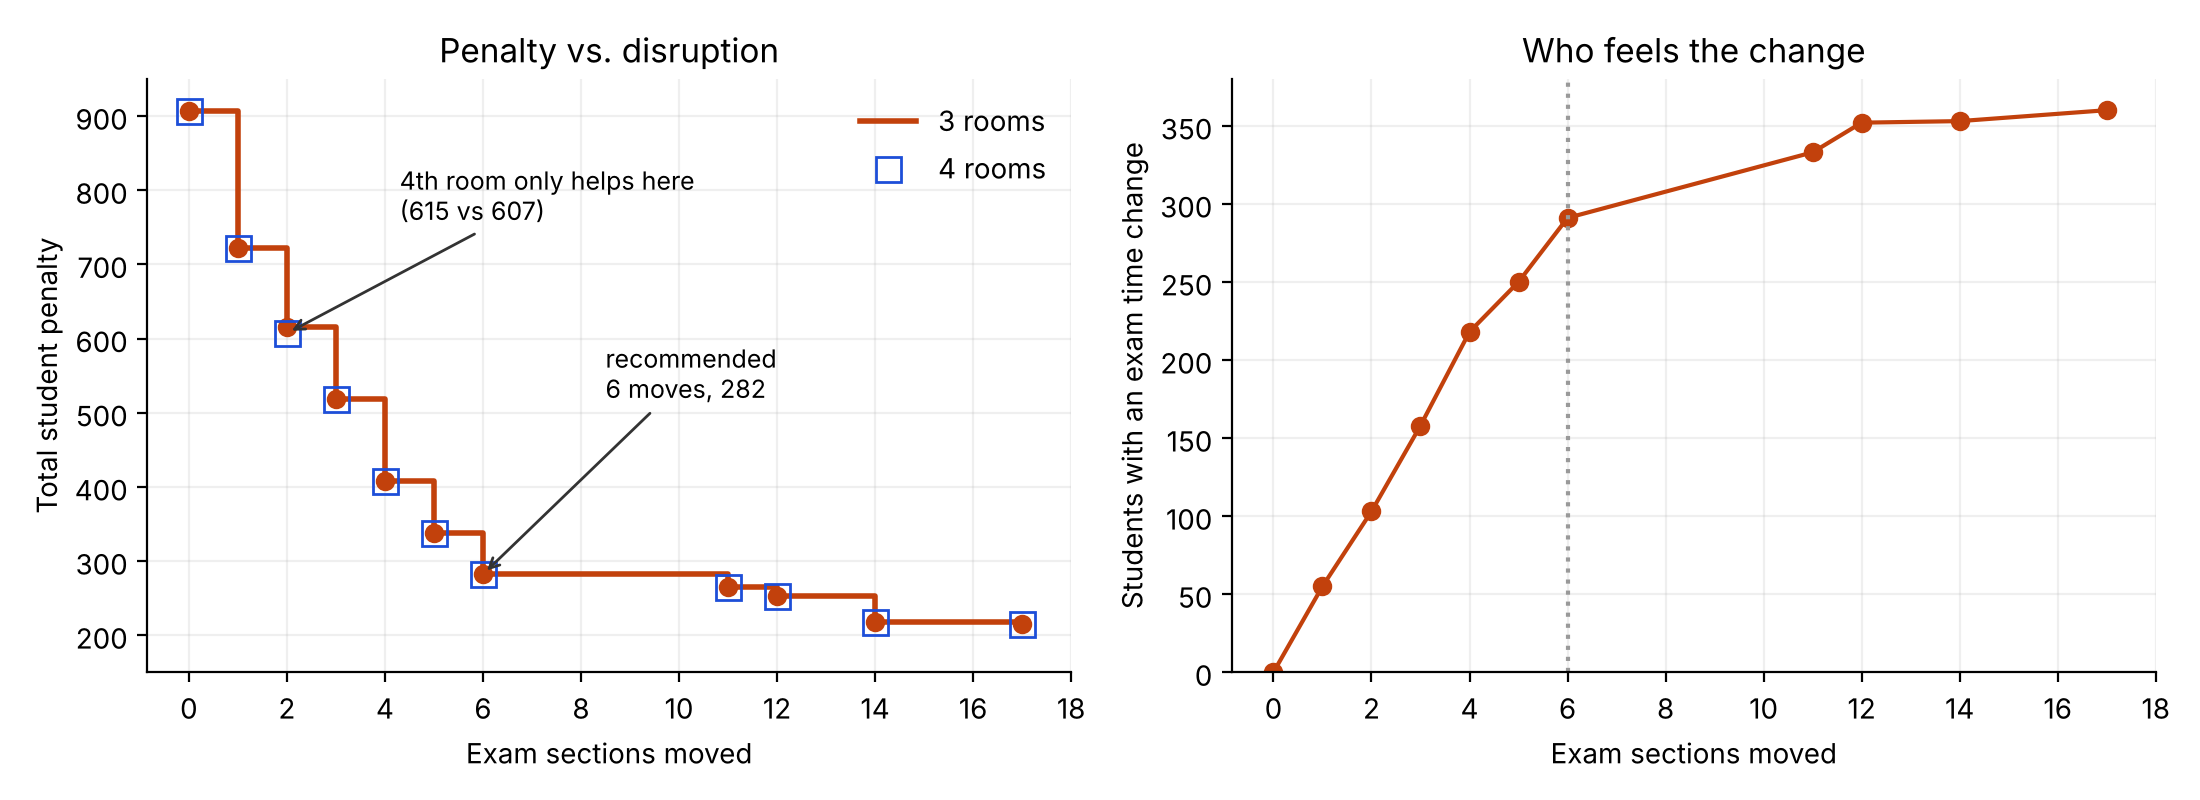
\includegraphics[width=0.74\linewidth]{../results/pareto.png}
\vspace{-1.6em}
\caption{Best workload and students with a time change vs.\ sections moved (3 rooms; squares = 4 rooms).}
\label{fig:pareto}
\end{figure}
\vspace{-1em}

\textbf{Recommendation: move 6 sections, keep 3 rooms.} Workload falls from 907 to 282 ($-69\%$, 90\% of the achievable gain) and every back to back is gone; the worst student drops from 8 to 4 and students penalized from 226 to 119. It clears Dec 17 at 8:00 and 11:20: 2028-B, 3044-B and 3104-B join their A sections earlier in the week in Klaus-1443, 3232-A moves to Dec 15, and 4034-A and 4111-A slide to 8:00; 3133-A only changes rooms. The cost is real: 291 of 360 students (81\%) see an exam time change. A 4-move schedule (408, 218 students affected, 28 back to backs left) is the fallback if time changes are judged more harmful.

\textbf{Extra room: not worth it.} The 3- and 4-room frontiers are identical except at 2 moves (615 vs 607). Same-course sharing in Klaus-1443 already frees the slots a fourth room would add; it would only matter if sharing were banned.

\textbf{Sensitivity.} Under the original weights (back to back 3, overnight 5) the same schedule still cuts workload from 827 to 434 ($-48\%$).

%--------------------------------------------------
\section{Limitations and AI disclosure}
Weights are subjective and total workload is not a full fairness measure. We do not capture instructors and TAs (grading load), proctors and room staff, students needing accommodations or makeups, or students outside the pilot. No cost is assigned to the fourth room. \textbf{AI use:} Temidayo used ChatGPT for model development, debugging, commands and documentation. Kelechi used Claude for the data loader, evaluator and audit code, git help, the report draft and the slide deck. Both of us ran all code, checked every reported number against the outputs, and are responsible for the submitted work.

\end{document}
